\documentclass[a4paper,14pt]{extarticle}
\usepackage[utf8]{inputenc}
\usepackage[english,russian]{babel}
\usepackage{amsmath,amsfonts,amsthm, mathtools}
\usepackage{amssymb}
\usepackage{graphicx}
\graphicspath{{images/}}
\usepackage{wrapfig}
\usepackage{floatrow}
\usepackage{setspace}
\usepackage[margin=10pt,font={small,stretch=0.9},labelfont=bf,labelsep=period,
justification=centerlast]{caption}
\usepackage{array,tabularx,tabulary,booktabs}
\RequirePackage{multirow}
\RequirePackage{multicol}
\RequirePackage{longtable}
\usepackage{indentfirst}
\usepackage{hyperref}
\usepackage{icomma}
\newcommand*{\hm}[1]{#1\nobreak\discretionary{}
	{\hbox{$\mathsurround=0pt #1$}}{}}
\usepackage{soulutf8} 
\usepackage{etoolbox} 
\usepackage{fancyhdr}
\renewcommand{\headrulewidth}{0mm} 
\cfoot{\thepage} 
\usepackage{geometry}
\geometry{top=20mm}
\geometry{bottom=20mm}
\geometry{left=20mm}
\geometry{right=20mm}
\DeclareMathOperator{\sgn}{\mathop{sgn}}

\begin{document}
	\begin{titlepage}
		\begin{center}
			\large Московский физико-технический институт\\
			(национальный исследовательский университет)\\
			\vspace{1cm}
			\begin{figure}[h!]
				\centering
				
\includegraphics[width=0.7\linewidth]{MIPT.jpeg}
				\label{fig:mpr}
			\end{figure}
			\vspace{3cm}
			\Large Вопрос по выбору \\
			\vspace{4cm}
			\textbf{\Huge <<Определение параметров оптического пучка методом лезвия>>}\\
		\end{center}
		
		\vspace{5cm}
		{\par \raggedleft \large Выполнил:\\ студент 1 курса ЛФИ \\ Сливка Глеб \par}
	\end{titlepage}
	\tableofcontents
	\newpage
	\section{Теоретические сведения}
	
\subsection{Уравнение гауссого пучка}
	
Рассмотрим праксиальную волну, её комплексная амплитуда записывается так: 
\begin{equation}
	u(\vec{r}) = A(\vec{r}) \exp(-jkz).
	\label{u(r)}
\end{equation}
	Одно из решений параксиального уравнения Гельмгольца приводит к гауссову пучку. Уравнение комплексной огибающей гауссого пучка: 
	\begin{equation}
		A(\vec{r}) = \frac{A_1}{q(z)} \exp \left( -jk \frac{\rho^2}{2q(z)} \right); \; \; \; q(z) = z + jz_0,
		\label{A(r)}
	\end{equation}
	где $q(z)$ --- q-параметр пучка, $z_0$ --- рэлеевская длина. Записав действительную и мнимую части комплексной функции получим: 
	
	\begin{equation}
		\frac{1}{q(z)} = \frac{1}{R(z)} - j \frac{\lambda}{\pi \omega^2(z)},
		\label{1/q}
	\end{equation}
	где $R$ --- радиус кривизны пучка, $\omega$ --- радиус пучка. Из \eqref{A(r)} и \eqref{1/q} получи выражения для комплексной амплитуды гауссого пучка: 
	\begin{equation}
		\boxed{u(\vec{r} ) = A_0 \frac{\omega_0}{\omega(z)} \exp \left[ \frac{-\rho^2}{\omega^2(z)}\right] \exp \left[ -jkz -jk \frac{\rho^2}{2R(z)}+ j \zeta(z) \right]}
	\end{equation}
	
	\begin{equation}
		\omega(z) = \omega_0 \sqrt{1 + \left(\frac{z}{z_0}\right)^2},
		\label{w(z)}
	\end{equation}
		\begin{equation}
			R(z) = z \left[1 + \left( \frac{z}{z_0}\right)^2 \right].
		\end{equation}
	\begin{figure}[H]
		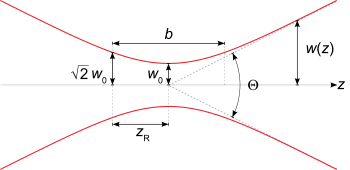
\includegraphics[scale=1]{beam}
	\end{figure}
 
	\subsection{Интенсивность}
	Оптическая интенсивность $I(\vec{r})= |u(\vec{r})|^2$ есть функция аксиальной $z$  и радиальной  $\rho = \sqrt{x^2 + y^2}$ координат точки: 

\begin{equation}
	I(\rho, z) = I_0 \left( \frac{\omega_0}{\omega(z)} \right)^2  \cdot \exp \left[ \frac{-2 \rho^2}{\omega^2(z)} \right].
	\label{I}
\end{equation}
	
	\begin{figure}[H]
		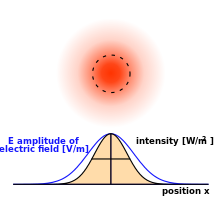
\includegraphics[scale=0.9]{I}
	\end{figure}

\subsection{Мощность}
Полная оптическая мощность, которую переносит луч, есть интеграл от интенсивности по любой поперечной плоскости: 

\begin{equation}
	P = \int_{o}^{\infty} I(\rho, z) 2 \pi \rho d\rho,
	\label{P}
\end{equation}	
вычислив получаем 
\begin{equation}
	P = \frac{1}{2} I_0 (\pi \omega_0^2).
\end{equation}

Таким образом зависимость интенсивности пучка выражается следующим образом: 

\begin{equation}
	\boxed{ I(\rho, z) = \frac{2P}{\pi \omega^2(z)} \exp \left[ \frac{-2 \rho^2}{\omega^2(z)} \right]}
	\label{IP}
\end{equation}

\subsection{Ширина пучка}

Так как интенсивность имеет гауссого распределение, то чётких границ у луча нет, поэтому чтобы определить радиус надо договориться. За радиус пучка принято принимать такое расстояние, при отступлении которого от центра пучка интенсивность падает в $1/e^2$ раз. Это расстояние равно $\rho = \omega$. 86 $\%$ мощности пучка переносится внутри этого круга. 

\end{document}